%% Este formato corresponde a la versi\'onn en espa\~nol de de la Revista MMSN
%% del Departamento de Matemtica de la Universidad Tecnolgica Metropolitana, de Santiago de Chile,
%% https://mmsb.utem.cl/.
%% Esta construido usando como base el formato de acceso abierto de la IEEE.

\documentclass[eng]{MMSB-class-eng}
\usepackage{color}
\spanishdecimal{.}%cambia la coma por el punto decimal

%%%%%%%%%%%%%%%%%%%%%%%%%%%%
% Page number where the article starts
%%%%%%%%%%%%%%%%%%%%%%%%%%%%
\setcounter{page}{1}


%%%%%%%%%%%%%%%%%%%%%%%%%%%%
% Publication title
%%%%%%%%%%%%%%%%%%%%%%%%%%%%
\title{Modeling macroparasite infection dynamics\\
{\ }\\
Modelizaci\'on de la dinámica de infecci\'on de macroparásitos}

%%%%%%%%%%%%%%%%%%%%%%%%%%%%
% Short title for the header (copy the main title if it is not too long)
%%%%%%%%%%%%%%%%%%%%%%%%%%%%
\shorttitle{Modeling macroparasite infection dynamics}

%%%%%%%%%%%%%%%%%%%%%%%%%%%%
% Authors
%%%%%%%%%%%%%%%%%%%%%%%%%%%%
\author[1,2]{Gonzalo Maximiliano Lopez}
\author[1]{Juan Pablo Aparicio}
%\author[1,2]{Benjam\'in Gonz\'alez Leiva}

%%%%%%%%%%%%%%%%%%%%%%%%%%%%
% Author Affiliations
%%%%%%%%%%%%%%%%%%%%%%%%%%%%
\affil[1]{Instituto de Investigaciones en Energ\'ia no Convencional, Consejo Nacional de Investigaciones Cient\'ificas y T\'ecnicas,
Universidad Nacional de Salta, Av. Bolivia 5150, 4400 Salta, Argentina}
\affil[2]{Departamento de Matem\'atica, Facultad de Ciencias Exactas, Universidad Nacional de Salta, Av. Bolivia 5150, 4400 Salta, Argentina}


%%%%%%%%%%%%%%%%%%%%%%%%%%%%
% Last name of the first author of the work
%%%%%%%%%%%%%%%%%%%%%%%%%%%%
\firstauthor{Lopez}

%%%%%%%%%%%%%%%%%%%%%%%%%%%%
% Contact author details
%%%%%%%%%%%%%%%%%%%%%%%%%%%%
\contactauthor{Lopez}
\email{gonzalo.maximiliano.lopez@gmail.com} 
%\mailingaddress{Las Palmeras 3360, \~Nu\~noa, Chile}
%\phonenumber{+56 2 2787 7522}

%%%%%%%%%%%%%%%%%%%%%%%%%%%%
% Publication data (will be defined in the edition)
%%%%%%%%%%%%%%%%%%%%%%%%%%%%
\thisvolume{XX}
\thisnumber{XX}
\thismonth{MES}
\thisyear{20XX}
\receptiondate{dd/mm/aaaa}
\acceptancedate{dd/mm/aaaa}
\publicationdate{dd/mm/aaaa}


%%%%%%%%%%%%%%%%%%%%%%%%%%%%
% Place your particular definitions here
%%%%%%%%%%%%%%%%%%%%%%%%%%%%
\newcommand{\vect}[1]{\mathbf{#1}}

%%%%%%%%%%%%%%%%%%%%%%%%%%%%
% Start document
%%%%%%%%%%%%%%%%%%%%%%%%%%%%
\begin{document}

%%%%%%%%%%%%%%%%%%%%%%%%%%%%
% Introduzca aquí el resumen en español
%%%%%%%%%%%%%%%%%%%%%%%%%%%%
\resumen{
En este trabajo presentamos un marco general para la modelizaci\'on de la dinámica de transmisión de macroparásitos que no se reproducen dentro del hospedador como \textit{Ascaris lumbricoides}, \textit{Trichuris trichiura}, \textit{Necator americanus} y \textit{Ancylostoma duodenal}. Los modelos básicos se derivan de modelos probabilísticos generales para la probabilidad de apareamiento denso-dependiente del parásito. Aquí consideramos el caso particular y común de una distribución binomial negativa para el número de parásitos en hospedadores. Encontramos el número reproductivo básico y mostramos que el sistema presenta una bifurcación nodo silla en algún valor del número reproductivo básico. También encontramos los equilibrios y el número básico de reproducción de un modelo para el caso más general de poblaciones heterogéneas de hospedadores.
}

%%%%%%%%%%%%%%%%%%%%%%%%%%%%
% Introduzca aquí las palabras clave en español
%%%%%%%%%%%%%%%%%%%%%%%%%%%%
\palabrasclave{Bifurcación nodo silla; Distribución binomial negativa; Macroparásito; Modelo matemático; Número reproductivo básico}

%%%%%%%%%%%%%%%%%%%%%%%%%%%%
% Insert here the abstract in English language
%%%%%%%%%%%%%%%%%%%%%%%%%%%%
\abstract{
In this work we present a general framework for the modeling of the transmission dynamics of macroparasites which do not reproduce within the host like \textit{Ascaris lumbricoides}, \textit{Trichuris trichiura}, \textit{Necator americanus} y \textit{Ancylostoma duodenale}.  
The basic models are derived from general probabilistic models for the parasite density-dependent mating probability. Here we considered the particular, and common case, of a negative binomial distribution for the number of parasites in hosts. We find the basic reproductive number  and we show that the system exhibits a saddle-node bifurcation at some value of the basic reproduction number. 
We also found the equilibria and basic reproduction number of a model for the more general case of heterogeneous host populations.
}

%%%%%%%%%%%%%%%%%%%%%%%%%%%%
% Insert here the keywords of your work in English language
%%%%%%%%%%%%%%%%%%%%%%%%%%%%
\keywords{Basic reproductive number; Macroparasite; Mathematical modeling; Negative binomial distribution; Saddle-node bifurcation}

%%%%%%%%%%%%%%%%%%%%%%%%%%%%
% Include title, authors, abstract, etc.
%%%%%%%%%%%%%%%%%%%%%%%%%%%%
\maketitle
\thispagestyle{fancy}
%\printcontactdata

%%%%%%%%%%%%%%%%%%%%%%%%%%%%
% Main body of work
%%%%%%%%%%%%%%%%%%%%%%%%%%%%
\newpage
\section{Introduction}
\primerapalabra{M}{athematical}% Letra capital en primera palabra
 models play an important role in understanding the transmission and impact of macroparasite diseases control measures \citep{anderson1992infectious,anderson2014coverage,truscott2016soil}.

The first works on the theory of helminth infection was published in the 1960's by Tallis and Leyton by developing stochastic models of nematode parasite transmission in sheep and cattle \citep{leyton1968stochastic,tallis1966stochastic,tallis1969stochastic}.

Simultaneously Macdonald show that a consequence of sexual reproduction of distributed parasites within individual hosts was the inability to generate fertile infectious material when prevalence is low \citep{macdonald1965dynamics}.


{\color{red}
Anderson and May introduced a much more general descriptions of helminth population dynamics based on host age, distribution of parasite numbers per host, density dependence of egg production, and sexual mating functions that depend on parasite distribution and reproductive habits \citep{anderson1982population,anderson1985helminth,anderson1992infectious}.
}

{\color{red}
In this article we develop an analytical framework to describe the transmission dynamics of most macroparasite infections. We show how the classical deterministic models are derived from probabilistic considerations about parasite distribution in hosts, egg production, and mating probability. 


We first describe the dynamics of infection transmission by macroparasites. 
Then we present two deterministic models for the transmission dynamics. The first model the simpler case of  a homogeneous host community while the second model the more complex case of a heterogeneous host community.
}

In both models, reproductive characteristics of the parasite are considered, such as egg production and mating probability, both modeled by the density-dependent fecundity of the parasite and the distribution of parasites per host, which we assume to be negative binomial.	


{\color{red}
For both models we computed the endemic equilibrium  and the basic reproduction number $R_0$, defined  as the average number of new parasite offspring produced by a typical 
%\color{blue} female?}  
female parasite, from one generation to the next. Finally  we show that the homogeneous model undergoes a saddle-node bifurcation. 
}

%{\color{blue} REFEREE: Introduction: I think that information is missing, for example, indicate:
%	
%	
%	- Problem to solve, principal objective or motivation
%	
%	
%	- Route of solution or response indicating the sections }

\section{General framework}

Microparasite diseases are usually modeled using compartmental models. After infection,  microparasite population may rapidly grow into the host. This intra-host parasite dynamics determines the level of infectiousness of the individual. In a simple compartmental  model like the $SIR$-model  all the susceptible individuals are grouped in one class of size $S$, all the infected and infectious individuals in a class of size $I$ and all the recovered individuals in a class of size $R$. Many refinements are possible, but the evolution of the parasite population within the host it is not considered or very simplified (for models including intra-host population dynamics 
see for example \citet{gandolfi2015epidemic}).
The most common refinement consists in dividing infected individuals in two classes, exposed (those infected but yet not infectious) and infectious, which leads to the well known $SEIR$ type models. 

\begin{figure}[!tb]
	\centering
	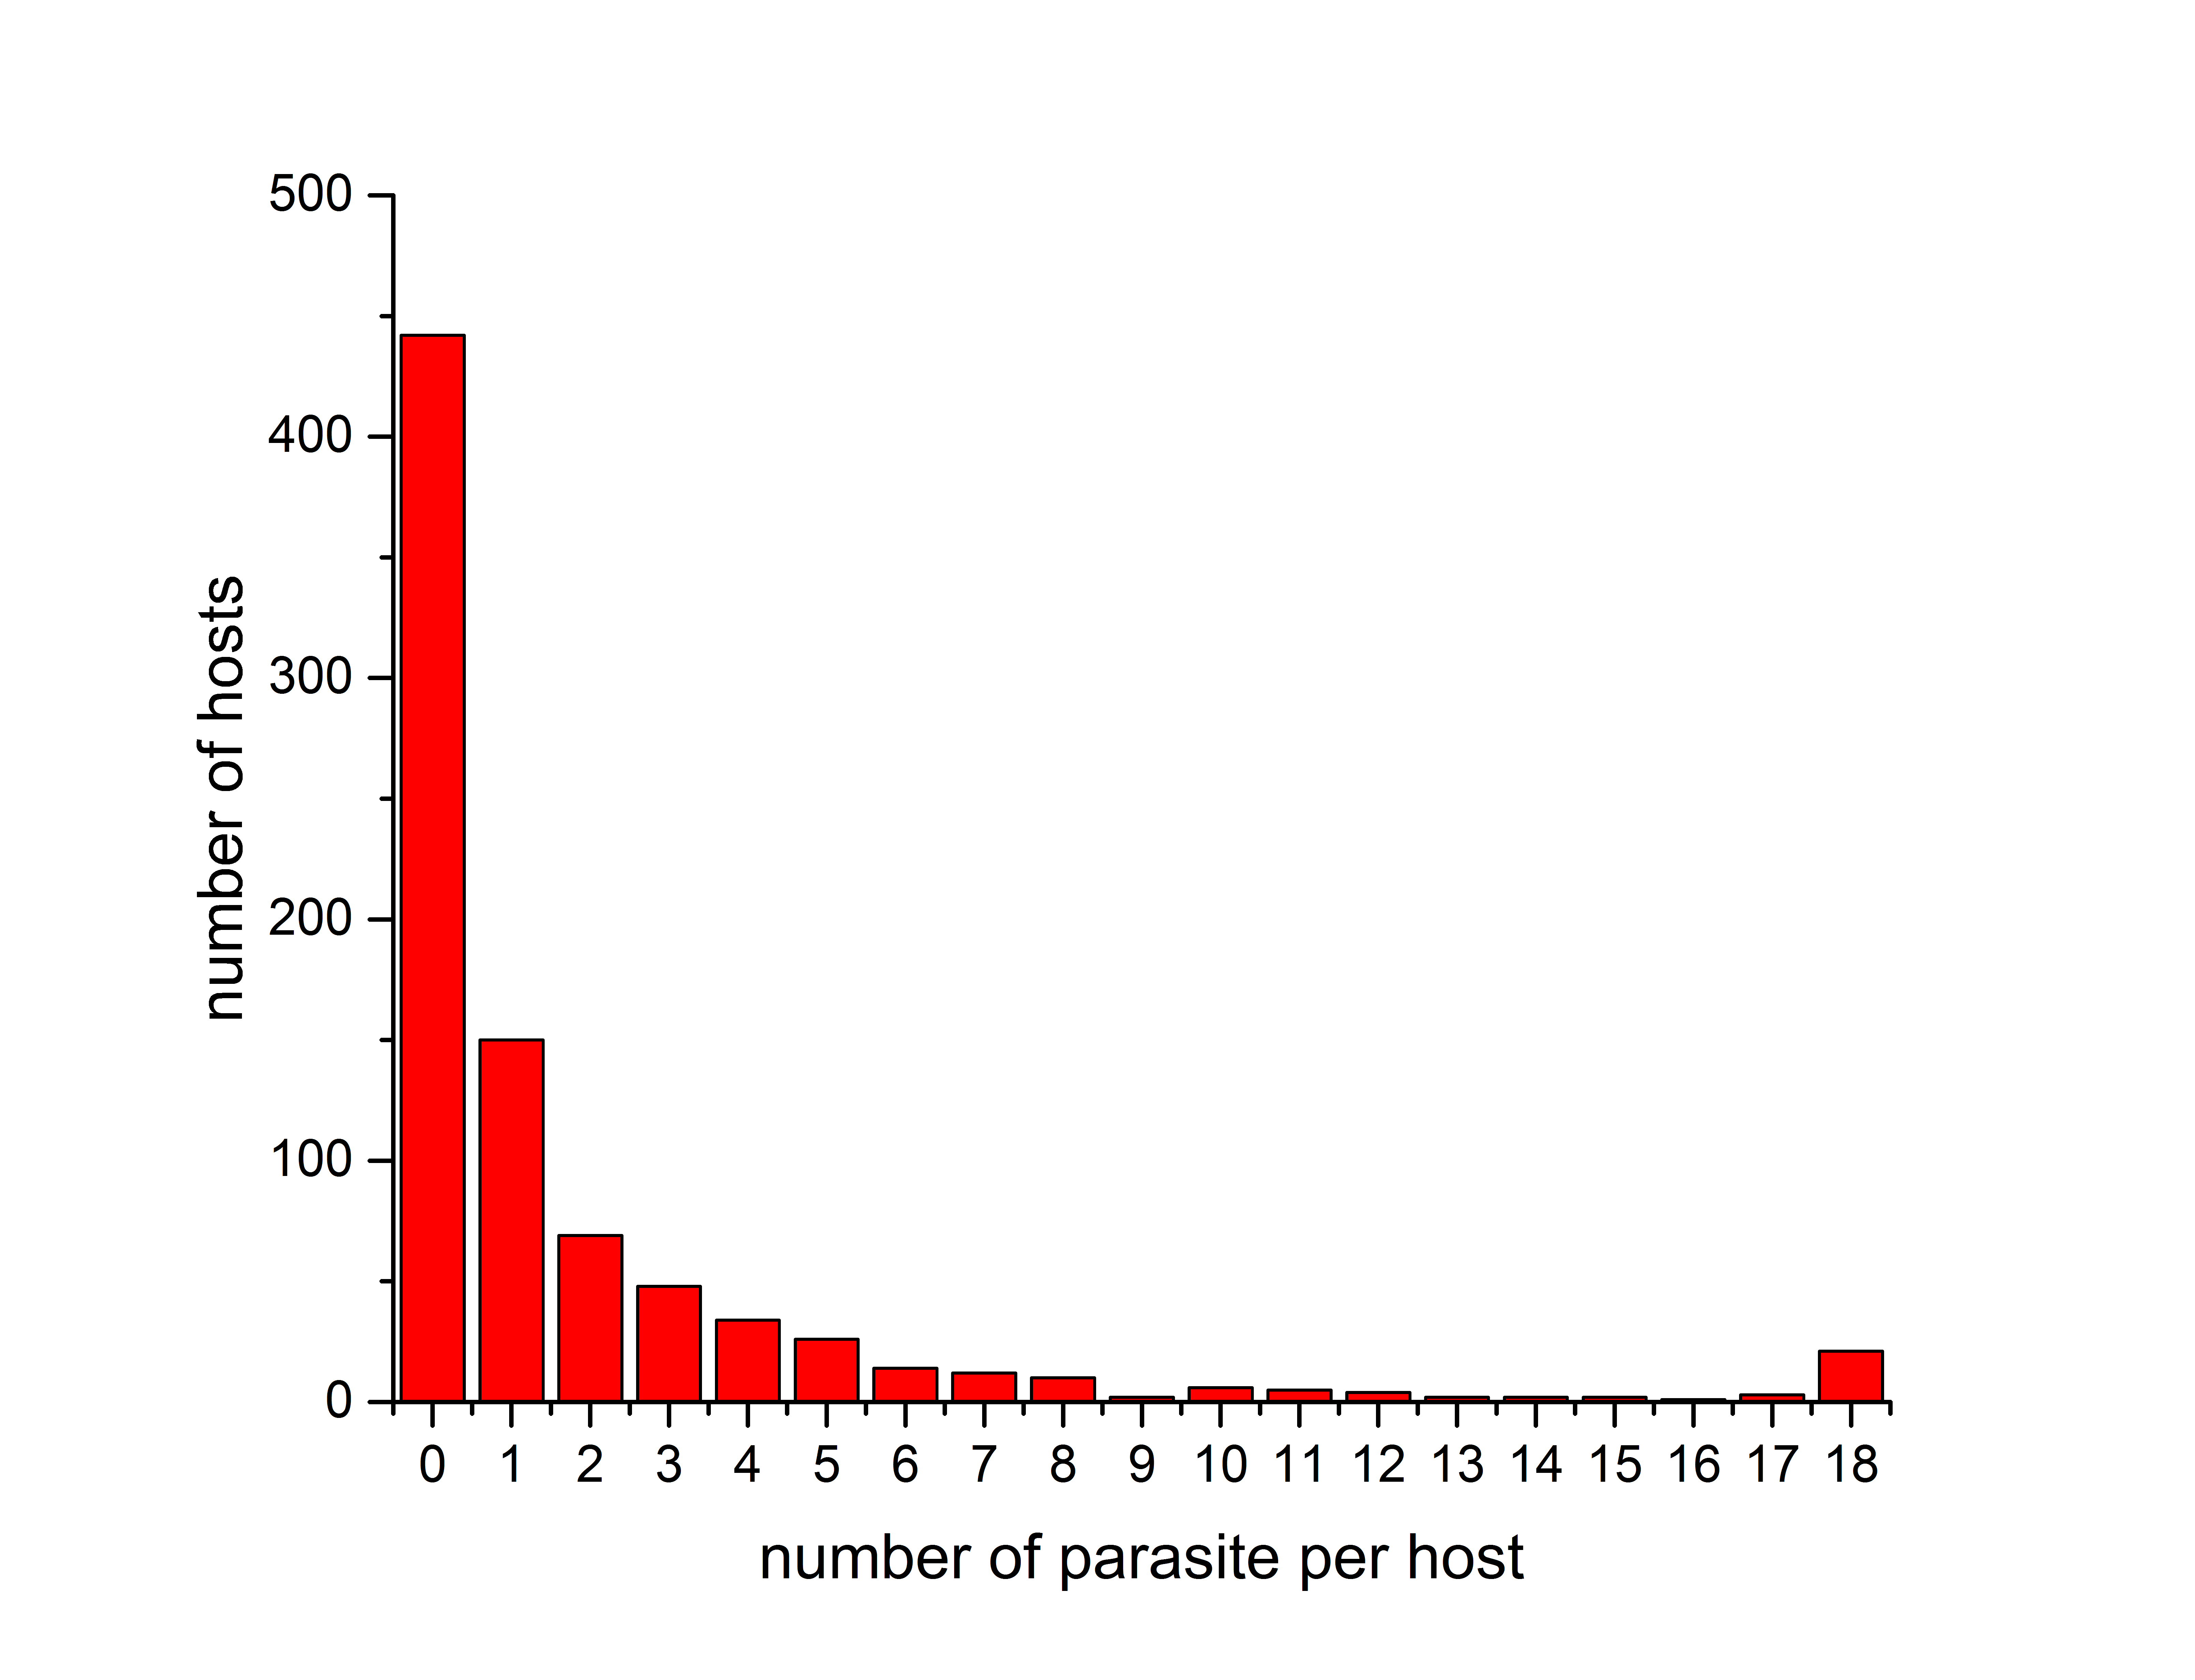
\includegraphics[width=0.99\linewidth]{dataseo}
	\caption{Distribution of \textit{Ascaris lumbricoides} parasite numbers per host in a study in rural populations in Korea \citep{seo1979frequency}. Most hosts are uninfected or infected with a low burden of parasites while few are infected by large numbers of parasites.}
	\label{fig:dataseo}
\end{figure}

For most macroparasites, the situation is completely different as these types of parasites do not reproduce within the host.  Most  infected  individuals have few macroparasites with a non-bell shaped distribution (see Figure \ref{fig:dataseo}) where few individuals concentrate most of the parasites in the host population \citep{seo1979frequency,lopez2022simple}. Negative binomial distributions usually provide a good description of the data. On the other hand, there is no host-to-host transmission of macroparasites as the life cycle completes in the environment (from where the host gets infected).  


Therefore the number of infected hosts is not a representative variable of the parasite burden. Simple models for macroparasites consider the evolution of the mean burden of parasite within the population as well as the environmental parasite reservoir (which is composed of eggs and/or larvae). From the mean burden, the total parasite population is easily estimated. 

%{\color{blue}REFEREE: General framework: Here, I consider the authors should connect it with the
%	objective or motivation of your proposal. Also, include comments about your
%	previous work cited as [9].}

\section{A basic model}
\label{s:basicmodel}

\subsection{Model structure}
\label{ss:structure}
The model presented in this paper is based on a model developed by Anderson and May \citep{anderson1992infectious}.
The conceptual framework of parasite transmission dynamics is conceptualized as a population of mature parasites within human hosts and a population of infective stages (eggs and/or larvae) found in the environment (reservoir).
Hosts may become infected by contact with the infective stages of the parasites 
and can contaminate the environment by releasing parasite's eggs to the environment (see Figure \ref{f:diagram}). 
\begin{figure}[h!]
	\centering
	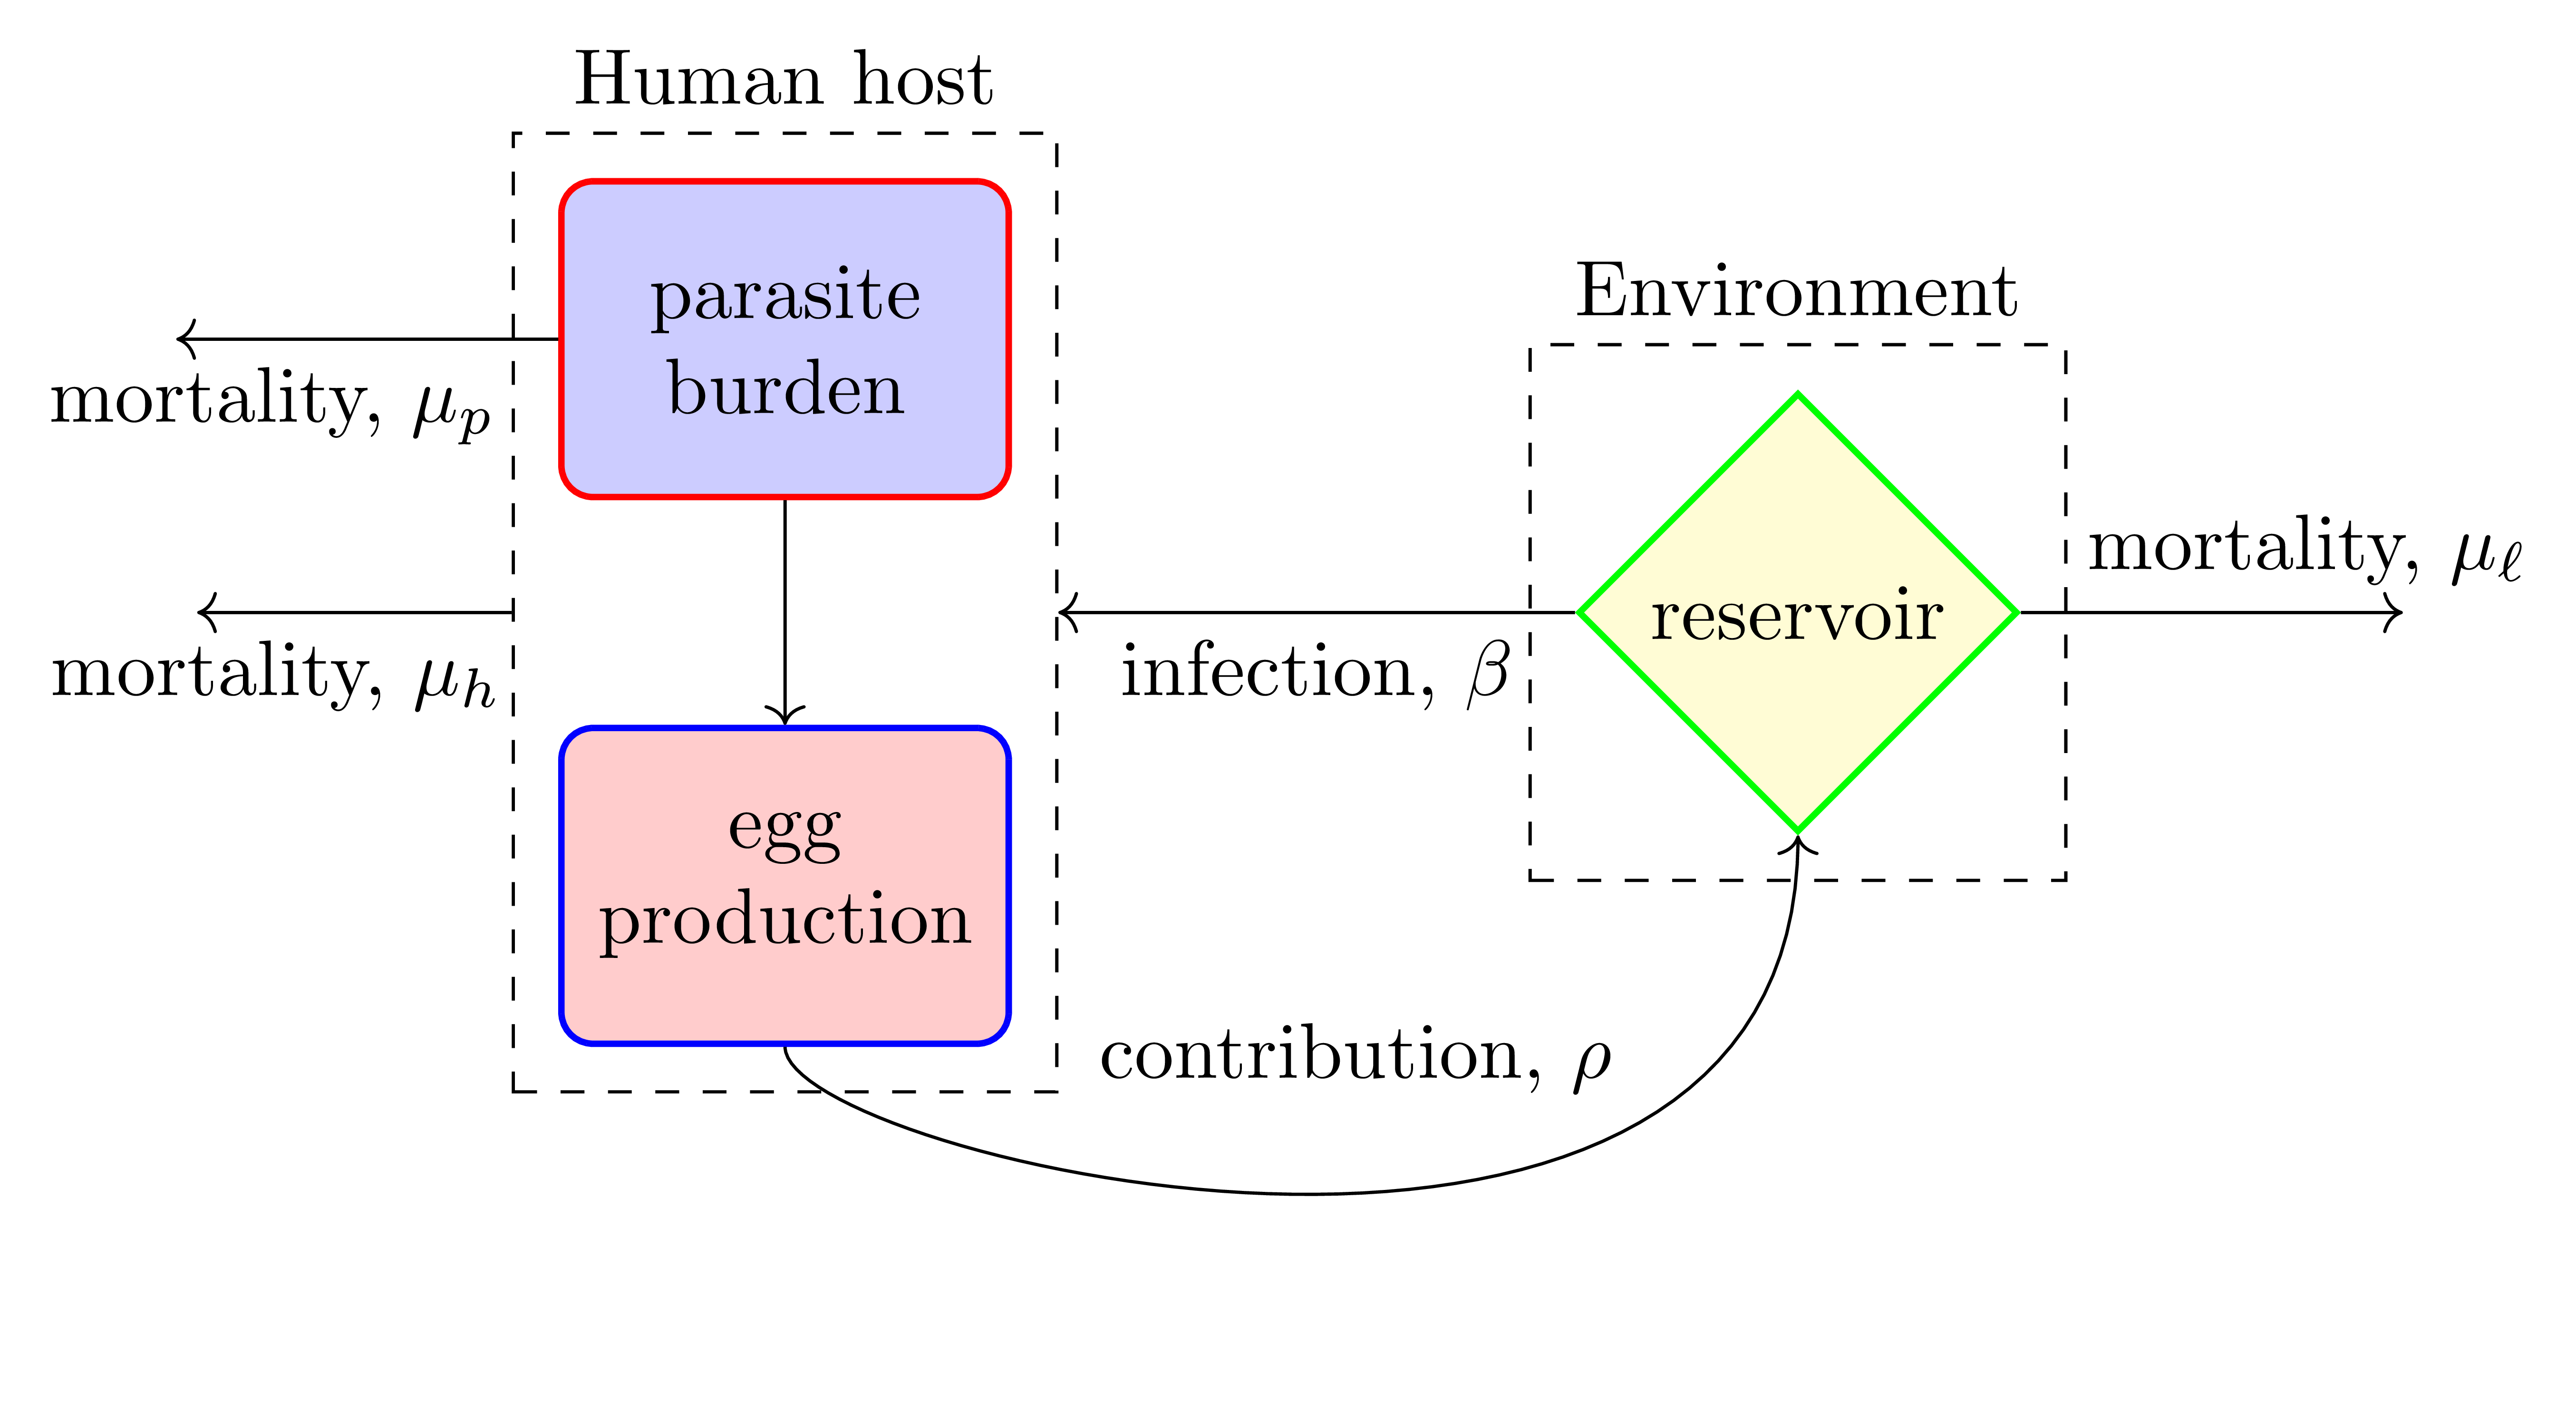
\includegraphics[width=0.99\linewidth]{diagram}
	\caption{Conceptual framework of parasite transmission dynamics.}
	\label{f:diagram}
\end{figure}

In a simple model for transmission dynamics of parasites, 
the dynamic variables  are the mean parasite burden in the host population, $m$; and the population of infective stages (reservoir) in the environment, formed by eggs and/or larvae, $\ell$. 

In the following we will sketch the procedure to find parasite-related parameters from a statistical-probabilistic model for the parasite population.

The environmental parasite reservoir, composed by eggs or larvae, increases due to the contribution of adult parasites within the hosts. As most hosts harbor only few parasites, only hosts with at least one female and one male parasites will contribute with fertilized eggs to the reservoir. We will consider that the random variable $W$, the number of parasites in a host, follows a negative binomial distribution. 
Therefore, the probability of observing $n$ parasites in a host is
\begin{equation}\label{disnb}
%\mathrm{P}(W=n)=\frac{\Gamma(k+n)}{\Gamma(n+1)\Gamma(k)}\left( \frac{k}{m+k}\right) ^{k} \left( \frac{m}{m+k}\right) ^n,
\mathrm{P}(W=n)=\frac{\Gamma(k+n)}{\Gamma(n+1)\Gamma(k)}p^{n}(1-p)^k,
\end{equation}
{\color{red}
where $\Gamma$ is the gamma function and $p=\frac{m}{m+k}$ with   
$m$ the mean value (the mean population parasite burden) and $k$ the shape parameter. The variance may be expressed in terms of  $m$ and  $k$ as $\sigma^2=m+m^2/k$. 
The term $p$ is the host's probability of acquiring a parasite  and $1-p$ is the probability of not acquiring a parasite, 
in each of $k+n$ Bernoulli experiments. 


Mean egg production depends on the number of parasites within the host, and it is a density-dependent process. 
A simple model for the mean female fecundity of a female parasite in competition with $n-1$ parasites is given by 
\begin{equation}
\lambda(n)=\lambda_0 z^{n-1},
\end{equation}
where $\lambda_0$ is the rate of egg production per female independent of parasite density in host and $z=e^{-\gamma}$ with $\gamma$ a parameter quantifying the intensity of the competition. A study of the \textit{Ascaris lumbricoides} fecundity is presented in \citet{hall2000geographical}. 


Using the parasite host distribution \eqref{disnb} we may compute the mean egg production per host as \citep{lopez2022general}
$\lambda_0
\alpha m
\psi(m,k,z)$
where $\alpha$  is the fraction of female parasites in a host and $\psi$, the average effective contribution per female parasite to the parasite reservoir (see \citet{churcher2006density,lopez2022general}), is given by}
\begin{equation}\label{psi}
\psi(m,k,z)=\left[ 1+(1-z)\dfrac{m}{k}\right]^{-(k+1)},
\end{equation}




However, only hosts with at least one female parasite and one male parasite will effectively contribute to the parasite reservoir by the production of fertilized (or infective) eggs. 
Therefore, the mean fertilized egg production per host is

\begin{equation}\label{meanfertilizedeggs}
\lambda_0
\alpha m
\psi(m,k,z)\phi(m,k,z),
\end{equation} 
where $\phi(m,k,z)$ is the mating probability for the negative binomial distribution \citet{lopez2022general}
\begin{equation}\label{phi}
\phi(m,k,z)=1-\left[ \frac{1+ \left( 1-
	%\dfrac{z}{2} 
	\alpha z
	\right) \dfrac{m}{k}}{1+(1-z)\dfrac{m}{k}}\right] ^{-(k+1)}.
\end{equation}
Therefore, the mean fertilized egg contribution to the environmental reservoir  per host and per unit of time is
$\rho\lambda_0
\alpha m
\psi(m,k,z) \phi(m,k,z)$ where $\rho$ 
is the host's own contribution rate and the total contribution of eggs to the reservoir per unit of time of a host population of size $N$ is 
$\rho\lambda_0
%\frac{m}{2} 
\alpha m
\psi(m,k,z) \phi(m,k,z) N$. 
%{\color{red} tenemos que poner $\rho$? o ya esta eso en $\lambda(n)$?, verlo)} 

{\color{red}
The population of eggs and/or larvae in the environment ($\ell$) also decreases due to egg/larval mortality (at the rate $\mu_{\ell}$) and due to host infection at the rate $\beta \ell$ per host, however, we consider this last term is negligible relative to the size of $\ell$. 
Therefore, the dynamics of the reservoir is given by
\begin{equation}\label{eqreservorioT}
\dfrac{d\ell}{dt}= \rho\lambda_0
%\frac{m}{2} 
\alpha m
\psi(m,k,z) \phi(m,k,z) N- \mu_{\ell} \ell.
\end{equation}

Finally, the dynamics for the mean parasite burden $m$ is obtained as follows. Parasites are taken from the environment at a rate $\beta N \ell $ and therefore, the mean parasite burden increases at a rate $\beta  N\ell/N=\beta\ell $. Parasites within the host die at a rate $\mu_p$ and hosts at a rate $\mu_h$ (killing all their parasites). Thus, the dynamics of $m$ is given by
\begin{equation}\label{eqm}
\dfrac{dm}{dt}=\beta \ell - (\mu_h+\mu_p)m.
\end{equation}

%Because an average host has contact with a small part of the environment L (by infection and contribution), we will consider  that the environment variable L, is the relative environment to a host, which is L/N. Thefore, the dynamic of the new variable L  is given by 


Because an average host has contact with a small part of the reservoir $\ell$ (by infection and contribution), we rename the  variable, relative reservoir to a host, $\ell/N$ to $\ell$.
Then, the dynamic of the new variable $\ell$ is given by 	
\begin{equation}\label{eqreservorio}
\dfrac{d\ell}{dt}= \rho\lambda_0
%\frac{m}{2} 
\alpha m
\psi(m,k,z) \phi(m,k,z) - \mu_{\ell} \ell.
\end{equation}
	
Therefore, the conceptual framework of parasite transmission dynamics is conceptualized as shown in Figure \ref{f:diagram}. A basic model of the transmission dynamics of macroparasite infection in a homogenous host population is given by the following the system of nonlinear ordinary differential equations
{\color{red} 
\begin{equation}\label{model1}
\begin{split}
\dfrac{dm}{dt}&=\beta \ell - (\mu_h+\mu_p)m,\\
\dfrac{d\ell}{dt}&= \rho\lambda_0
\alpha m
\psi(m,k,z) \phi(m,k,z) - \mu_{\ell} \ell .
\end{split}
\end{equation}
}

\subsection{Equilibria and basic reproduction number}



{\color{red}
In this section we find some useful expressions involving the equilibrium values of the dynamical variables and the basic reproduction number $R_0$ defined as 
the average number of female offspring produced per female adult worm, that survive to reproductive maturity in the
absence of density-dependent constraints on parasite population growth \citep{anderson1992infectious}. Assuming the mating probability ($\phi$) and mean fertilized egg production ($\psi$) equal to one (this is an usual, but somewhat strong assumption, which will be discussed elsewhere), an average female parasite would release $ \lambda_0  \rho$ per unit of time to the environment. As the mean life of a parasite is approximately $1/(\mu_h+\mu_p)$ the total contribution of fertilized eggs become $\frac{\lambda_0  \rho}{ (\mu_h + \mu_p)}$. On the other hand, female parasites in hosts increase as the rate $\alpha\beta$ during an average time $1/\mu_{\ell}$. Therefore, the basic reproduction number is \citep{anderson1992infectious}
\color{red}
\begin{equation}\label{valorR0}
R_0=\frac{ \lambda_0 \alpha  \rho \beta }{\mu_{\ell} (\mu_h + \mu_p) },
\end{equation}
}

From the equation \eqref{eqreservorio} we obtain that at equilibrium
\begin{equation}\label{eqL}
\ell^*=\frac{ \lambda_0 \alpha}{\mu_{\ell}} \rho  m \psi(m)\phi(m), 
\end{equation} 
and substituting \eqref{eqL} in equation \eqref{eqm} we obtain the following equation for the dynamics of the mean parasite burden $m$
\begin{align}\label{eqMR0}
\dfrac{dm}{dt}&=(\mu_h + \mu_p)\left[ R_0  \psi(m)\phi(m) -1 \right] m,%\notag es para no tener numero en ecuacion
\end{align}


Therefore from the equation \eqref{eqMR0}, the mean parasite burden ($m^*$) satisfy
\begin{equation}\label{eqequilibrio}
\psi(m^*,k,z)\phi(m^*,k,z)=1/R_0.
\end{equation}
This equation presents two  equilibrium solutions for the mean parasite burden. 

As shown in the next section,  the dynamic system \eqref{model1} presents a saddle-node bifurcation.
The bifurcation occurs at the point $(m^b, R_0^b)$ where
\begin{equation}\label{meq}
\begin{split}
m^b=&\dfrac{k\left( \frac{1-\alpha z}{1-z}\right)^{\frac{1}{k+2}} - k}{(z-1)\left( \frac{1-\alpha z}{1-z}\right)^{\frac{1}{k+2}} + (1-\alpha z)},\\ R_0^b=&\left[ \psi(m^b;k,z)\phi(m^b;k,z)\right]^{-1}.
\end{split}	
\end{equation}
Therefore, for $R_0 > R_0^b$ there are three equilibria in the dynamic system \eqref{model1} (see Figure \ref{f:phase}),

\begin{itemize}
	\item An equilibrium is the \textit{\textbf{disease-free equilibrium}} present at $m^*= 0$, which is the trivial solution of equation (\ref{eqMR0}). 
	This equilibrium is an attractor for all values of $R_0$.
	
	\item The other equilibrium
	%One of the solutions 
	is the \textit{\textbf{endemic equilibrium}}, which is one solution of equation (\ref{eqequilibrio}).
	This equilibrium is an attractor for a range of values of $R_0> R_0^b $.
	
	\item The last equilibrium is an \textit{\textbf{unstable equilibrium}} and corresponds to the other solution of equation (\ref{eqequilibrio}).
	This equilibrium is a repulsor in the phase plane, that is, a barrier where values of $m(t)$ above the unstable equilibrium are attracted towards the endemic equilibrium and values of $m(t)$ below the unstable equilibrium are attracted to the disease-free equilibrium.

\end{itemize}
\begin{figure}[h!]
	\centering
	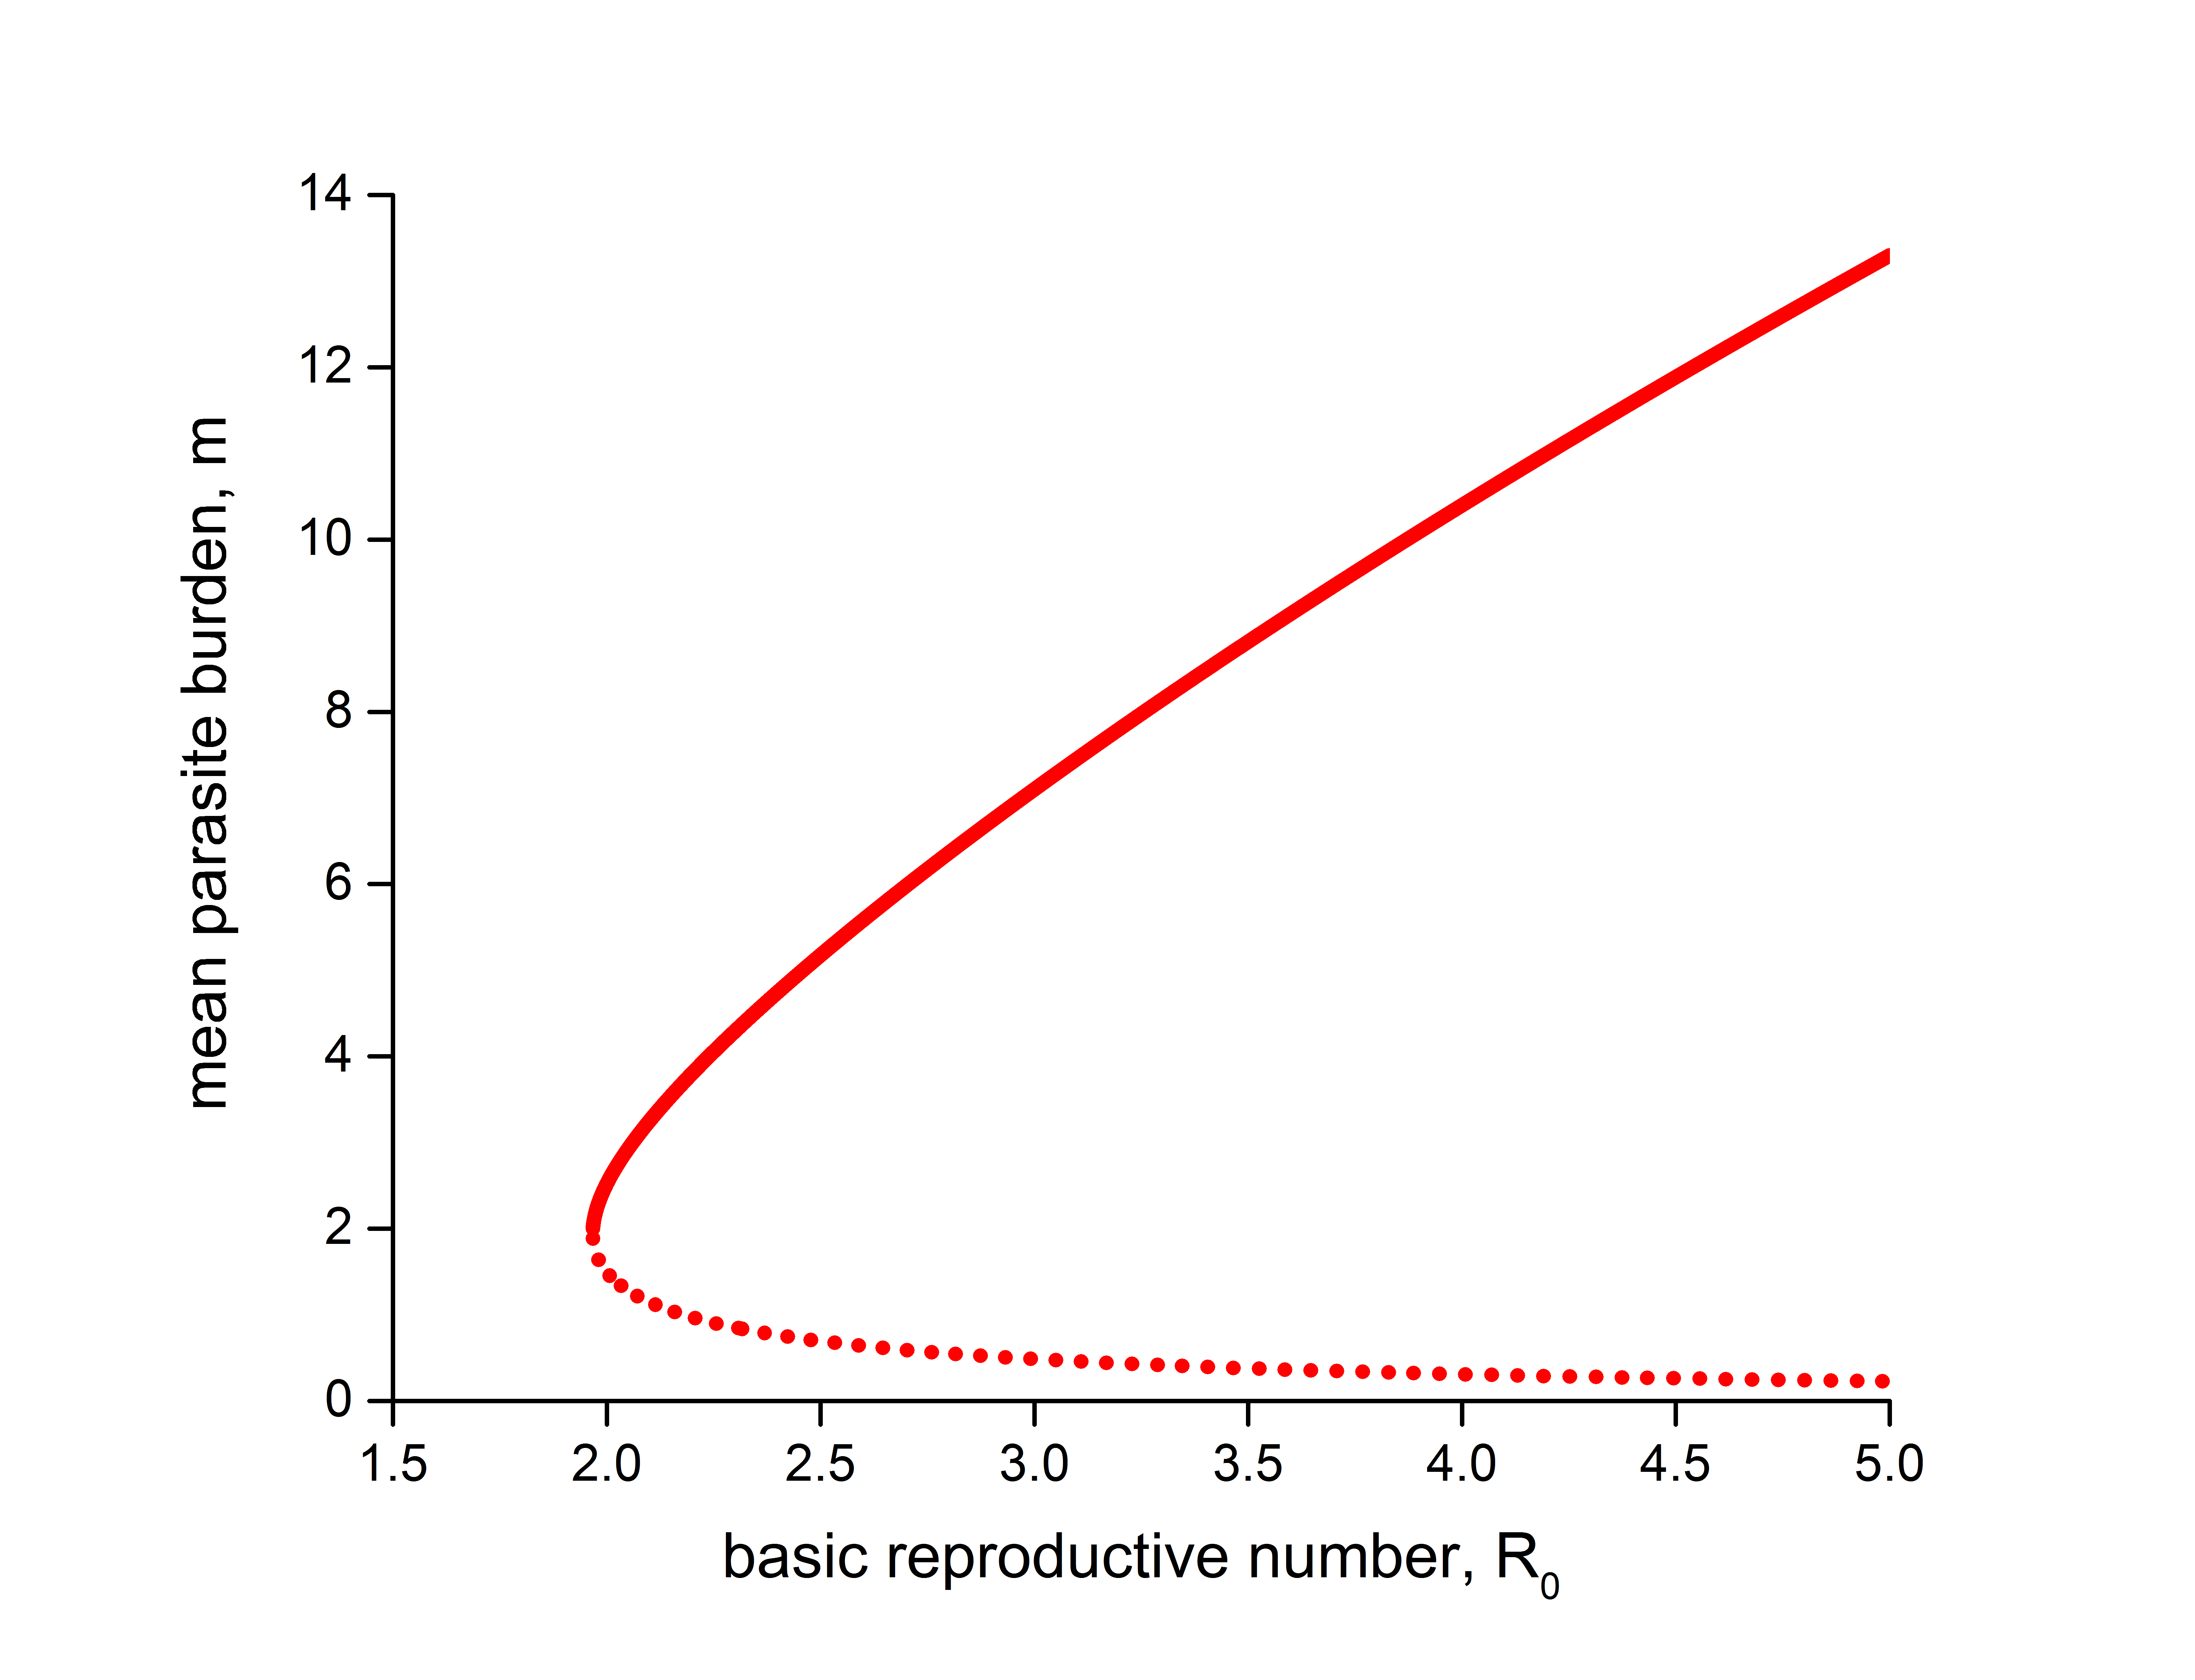
\includegraphics[width=0.99\linewidth]{bifurcation}
	\caption{Saddle-node bifurcation generated by eq. \eqref{eqequilibrio}, parameter values $\alpha=0.57$, $k=0.7$ and $z=0.93$.
	The solid line and dotted line correspond to the stable and unstable branch, respectively.}
	\label{f:phase}
\end{figure}

}



\subsection{Dynamics and bifurcation analysis}\label{bifurcacion}

{\color{blue}
 Dynamics of the reservoir is much faster than the parasite-host dynamics. This fact allows for a simplification by adiabatic elimination, that is we may assume that the dynamical variable $\ell$ is at a equilibrium at all times and therefore the two dimensional system \eqref{model1} reduces to the one-dimensional system 
\begin{equation*}
\dfrac{dm}{dt}=(\mu_h + \mu_p)\left[ R_0  \psi(m)\phi(m) -1 \right] m,
\end{equation*}
which we compactly denote by
$\dfrac{dm}{dt}=f(m,R_0)$.
This system undergoes a saddle-node bifurcation. 
A necessary condition for the existence of a such bifurcation at 
$(m^{b},R_0^b)$ is
\begin{equation}\label{conditionmbifur}
\begin{split}
f(m^b,R_0^b)&=0,\\
\dfrac{\partial f}{\partial m}(m^b,R_0^b)&=0,
\end{split}
\end{equation}
where the first of these conditions is the equilibrium condition \eqref{eqequilibrio} of the dynamic system
%donde la primera de estas condiciones es la condición de equilibrio (\ref{eqequilibrio}) del sistema 
\begin{equation*}
\psi(m^b;k,z)\phi(m^b;k,z)=1/R_0^b,
\end{equation*}
and using the second condition of \eqref{conditionmbifur} we obtain the following equation for $m^b$
%and so we get the following equilibrium condition for $\tilde m$
%y así obtenemos la siguiente condición para el equilibrio $m^{\star}$
\begin{equation}
\frac{\partial }{m}\psi(m^b;k,z)\phi(m^b;k,z)=0,	
\end{equation}
The value of $m^b$ corresponding to this last condition is
%El valor de $m$ correspondiente con esta ultima condición es 
\begin{equation}
m^b=\dfrac{k\left( \frac{1-\alpha z}{1-z}\right)^{\frac{1}{k+2}} - k}{-(1-z)\left( \frac{1-\alpha z}{1-z}\right)^{\frac{1}{k+2}} + (1-\alpha z)},	
\end{equation}
and its corresponding basic reproductive number is
%y el número reproductivo básico correspondiente es  
\begin{equation}
R_0^b=\left[ \psi(m^b;z,k)\phi(m^b;z,k)\right]^{-1},
\end{equation}	

A sufficient condition for the existence of a saddle-node bifurcation at $(m^b,R_0^b)$ is
\begin{equation}
\begin{split}
\dfrac{\partial f }{\partial R_0}(m^b,R_0^b)\neq0\\
\dfrac{\partial^2 f }{\partial m^2}(m^b,R_0^b)\neq0
\end{split}
\end{equation}

By a Taylor series expansion of the function $f$ in a neighborhood of $(m^b,R_0^b)$, the equation (\ref{eqMR0}) is given by
%\begin{equation}
\begin{multline}
%{\scriptstyle	
	\frac{dm}{dt}=f(m^b,R_0^b)+(m-m^b)\frac{\partial f }{\partial m}\big\vert_{(m^b,R_0^b)}\\ 
	+(R_0-R_0^b){\frac{\partial f }{\partial R_0}\big\vert_{(m^b,R_0^b)}}\\%\delta R_0
+{\frac {1}{2}}(m-m^b)^2{\frac{\partial^2 f }{\partial m^2}}\big\vert_{(m^b,R_0^b)}%\delta M^{2}
	+\cdots 
%}
\end{multline}
%\end{equation}
%Por lo tanto localmente en el punto $(m^{\star},R_0^{\star})$ la ecuación es de la forma
Therefore locally at the point $(m^b,R_0^b)$ the equation is of the form
\begin{equation}
\dfrac{dm}{dt}=A(R_0- R_0^b)+B(m- m^b)^2,
\end{equation}
where the values $A$ and $B$ are
\begin{equation}
A=(\mu_h +\mu_p)\frac{ m^b}{ R_0^b}, \qquad  B=(\mu_h + \mu_p) R_0^b  m^b \frac{\partial^2 F}{\partial m^2}( m^b),
\end{equation}
with $F(m)= \psi(m,z,k)\phi(m,z, k)$,
which is the normal form of a saddle-node bifurcation.

{\color{blue}
As a result of the above, we can obtain the following result
\begin{theorem}
	The model \eqref{model1} exhibits a saddle node bifurcation at the point $(m^b,R_0^b)$, if $R_0 \geq R_0^b$.
\end{theorem}
}

}


\subsection{Sensitivity analysis}
	
	{\color{red}	
		The transmission of macroparasitic diseases is related to the value of $R_0$. To predict which parameters have a higher impact on $R_0$, we may perform a sensitivity analysis on $R_0$.	
	
	The elasticity index o normalized sensitivity index measures the relative change of $R_0$ with respect to a parameter $x$, denoted by $\Gamma^{R_0}_{x}$, and defined as (see \citet{van2017reproduction})
	\begin{equation}
	\Gamma^{R_0}_{x}=\dfrac{\partial R_0}{\partial x} \dfrac{x}{R_0},
	\end{equation}
	The sign of $\Gamma^{R_0}_{x}$ tells us whether $R_0$ correlates positively or negatively  with the  parameter $x$; whereas its magnitude determines the relative importance of the parameter.
	
	For this model, the calculation of the elasticity indices are given by	
	%	The relative importance of each parameter for control measures can be estimated by computing elasticity indices. For this model,
	\begin{equation}
	\begin{split}
	\Gamma^{R_0}_{\lambda_0}&=\Gamma^{R_0}_{\alpha}=\Gamma^{R_0}_{\rho}=\Gamma^{R_0}_{\beta}=1,\\ 
	\Gamma^{R_0}_{\mu_{\ell}}&=-1,\\
	%\quad 
	\Gamma^{R_0}_{\mu_h}&=-\dfrac{\mu_h}{\mu_{h}+\mu_p},\\
	%\qquad 
	\Gamma^{R_0}_{\mu_p}&=-\dfrac{\mu_p}{\mu_{h}+\mu_p},
	\end{split}
	\end{equation}
	if $\frac{1}{\mu_h} \gg \frac{1}{\mu_p}$, then $\Gamma^{R_0}_{\mu_p}\approx -1$
	and 
	$\Gamma^{R_0}_{\mu_h}\approx 0$.
	In Figure \ref{fig:sensitivity} illustrated the sensitivity indices of $R_0$ which were obtained and evaluated using parameter values 
	%In Figure \ref{fig:sensitivity} illustrated the sensitivity index of $R0$ which were obtained and evaluated using parameter values 
	$\mu_h=\frac{1}{70}$ and $\mu_p=1$.
	\begin{figure}[h!]
		\centering
		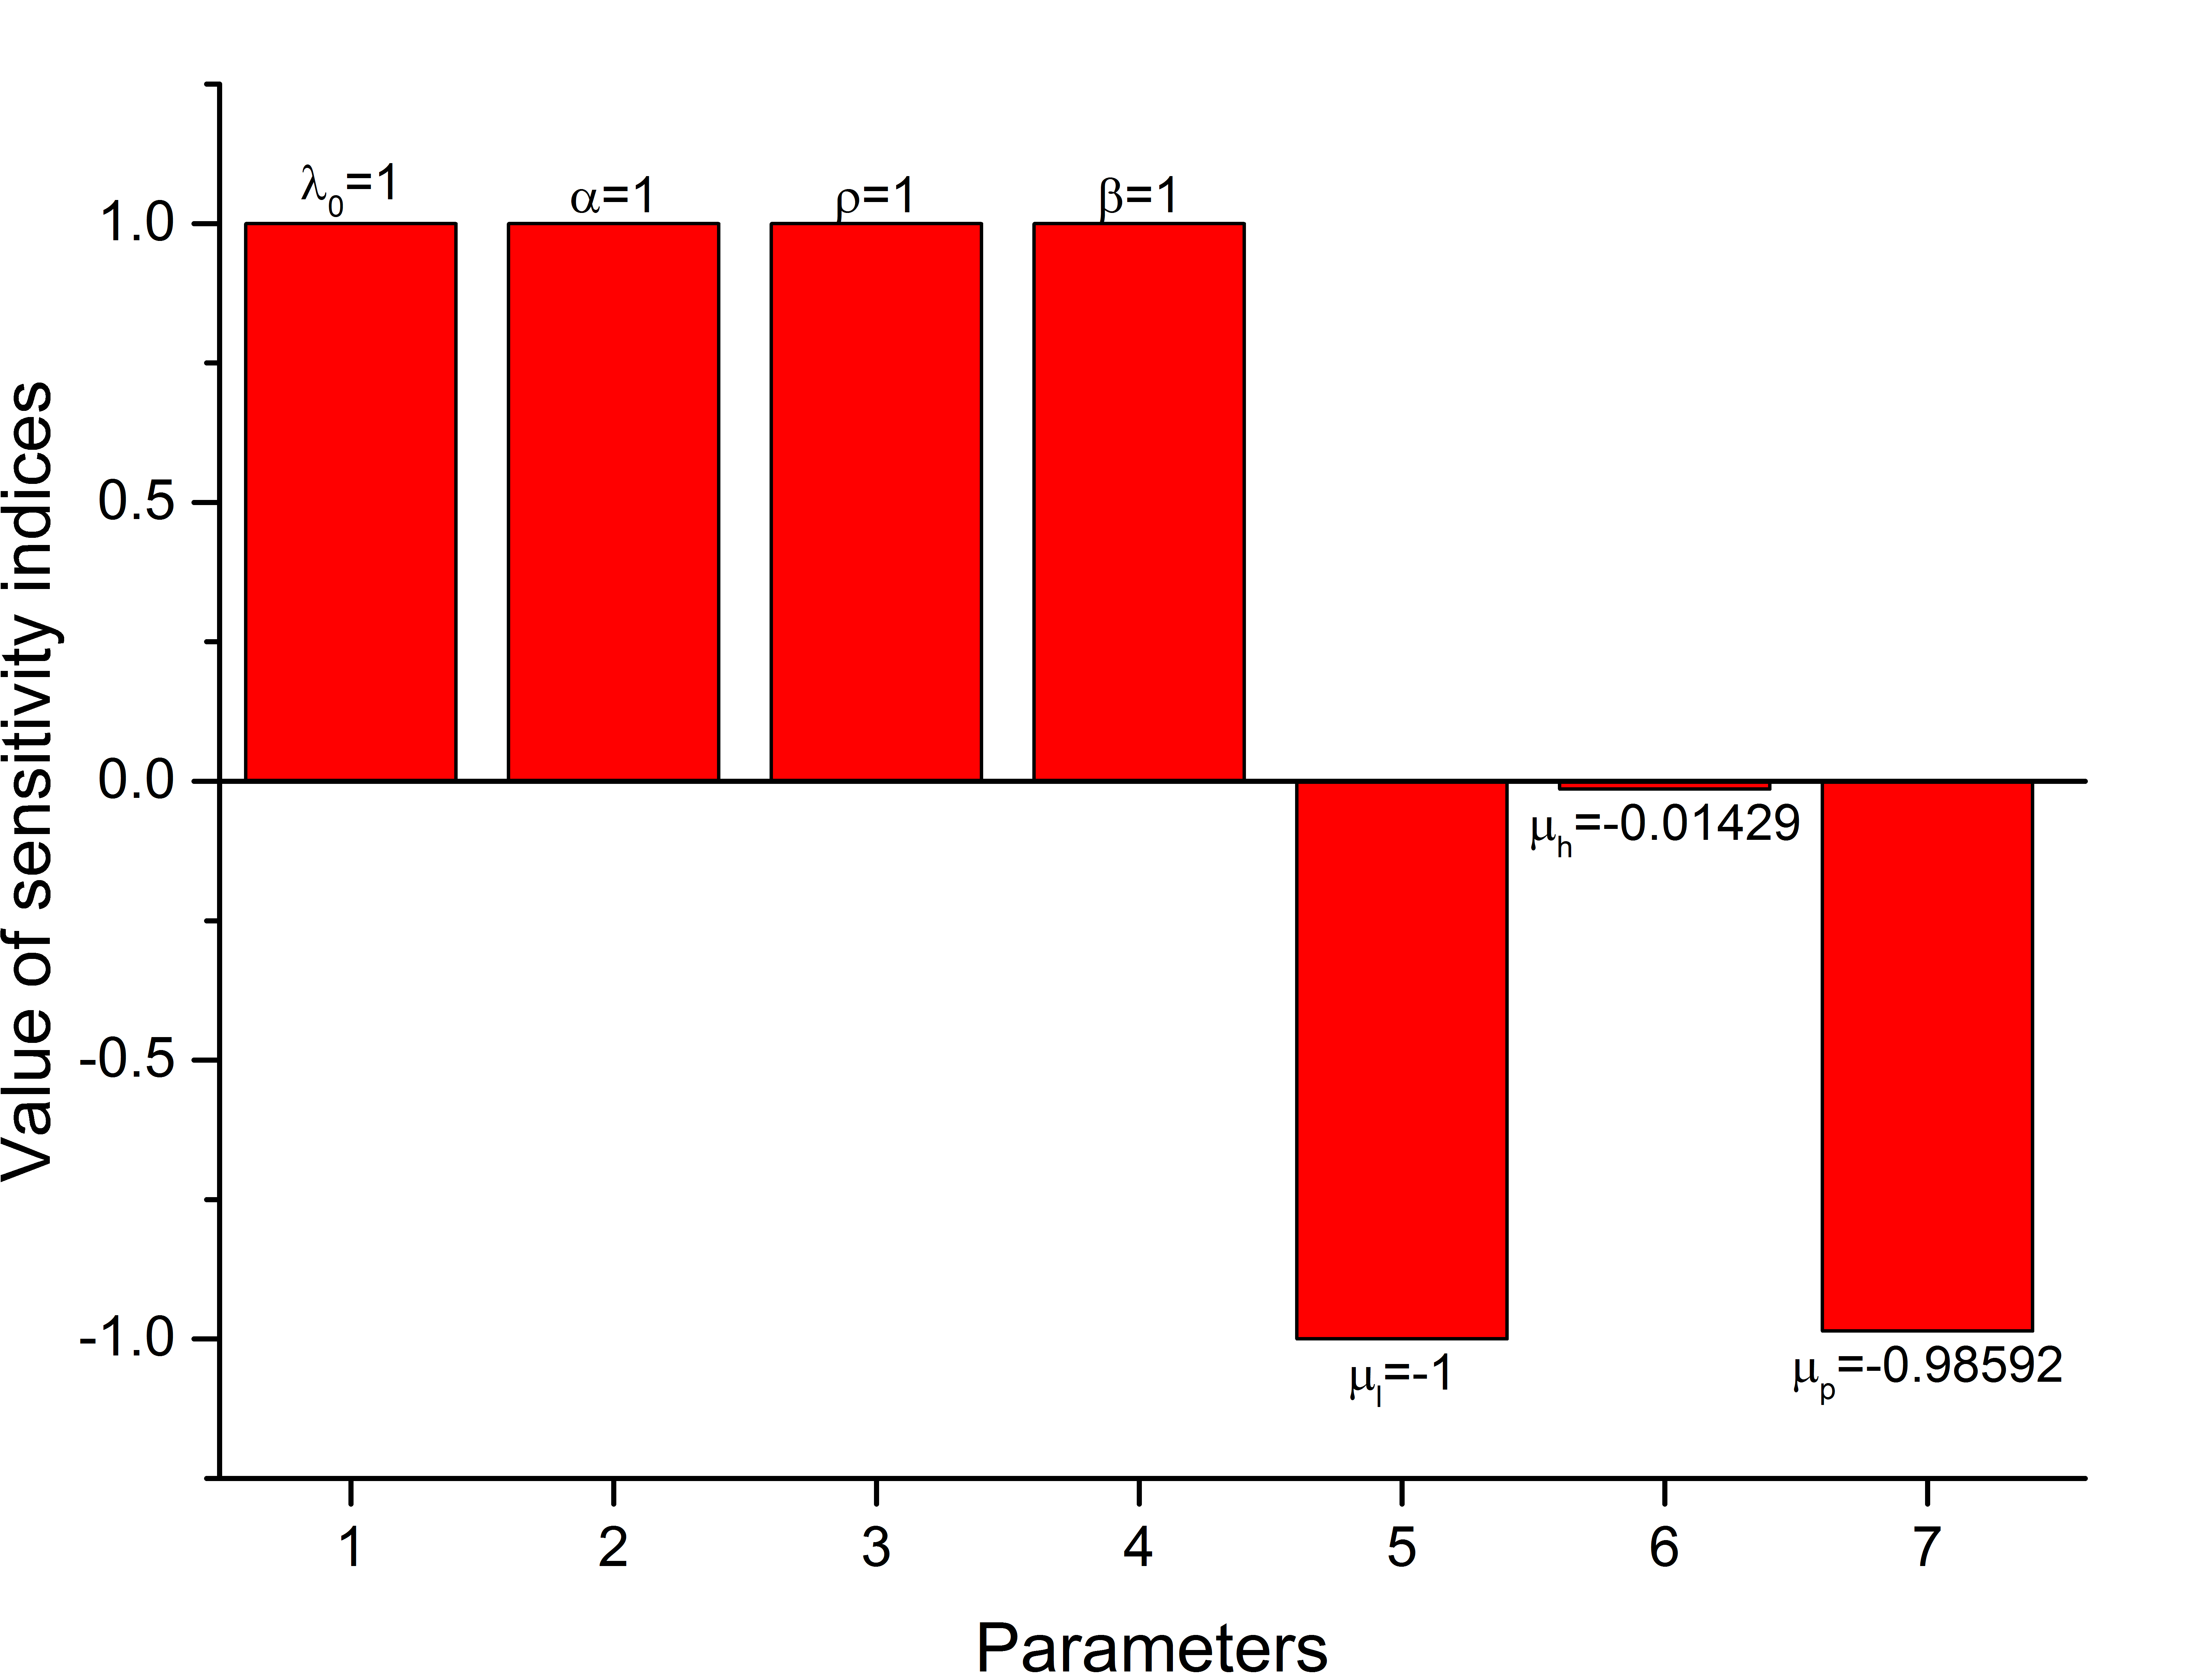
\includegraphics[width=0.9\linewidth]{sensitivity}
		\caption{Sensitivity analysis for $R_0$ with respect to each model parameter.}
		\label{fig:sensitivity}
	\end{figure}
	
	Clearly the most sensitive parameters for $R_0$ are $\lambda_0$, $\alpha$, $\rho$, $\beta$, $\mu_{\ell}$ and $\mu_p$.
	However, $\lambda_0$, $\alpha$ and $\mu_{\ell}$ correspond to parameters related to the life-cycle of the parasite which are quite difficult to modify, so a control measure for macroparasitic diseases should target  the reduction of $\rho$ and $\beta$, and the increase of $\mu_p$.
	
	Therefore, we can conclude from this analysis that the reduction of $R_0$ 
	is possible by reducing the egg contribution from the hosts to the reservoir, for example, by building latrines in the host community 
	or by reducing the infection from the reservoir to the hosts, for example, by washing hands and personal hygiene,  
	or by increasing parasite mortality, for example, through the application of periodic and specific antiparasitic treatments.	
	
	%is possible by reducing the egg contribution from the hosts to the reservoir, for example, by building latrines in the host community 
	%or by reducing the reduction from the hosts to the reservoir, for example, by by increasing parasite mortality, for example, through the application of periodic and specific antiparasitic treatments.	
	
}


\section{A heterogeneous model}
{\color{red}
In this section, we consider the most general and realistic case of a heterogenous host population. 

For this model, we assume that the host population, $H$, is divided into subpopulations, or groups, $H_i$, which present different characteristics, and therefore different risks of infection (for example, by age differential susceptibility, environmental conditions, access to sanitation and hygiene, etc.) 
\cite{anderson1992infectious,anderson2014coverage,brooker2006contrasting,freeman2015associations,truscott2014modeling}).

The dynamics of parasitic infection for the case of a heterogeneous population is described as follows:
\begin{equation}\label{model2}
\begin{split}
\dfrac{dm_i}{dt}&=\beta_i \ell - (\mu_h+\mu_p) m_i,\\
\dfrac{d\ell}{dt}&= 
%\frac{\lambda_0}{2}    
\lambda_0 \alpha
\sum_i  \pi_i \rho_i  m_i F(m_i)   - \mu_{\ell} \ell ,
\end{split}
\end{equation} 
where $i=1,\ldots,n$ with $n$ the number of groups in $H$ .     
The other parameters corresponding to each group $H_i$ are detailed in the following

\begin{itemize}
	\item $m_i$ is the mean parasite burden,
	\item $\beta_i$ and $\rho_i$  are the rate of contact (or exposure) and the rate of contribution
	of a host to the reservoir $\ell$, respectively,
	\item $N_{i}$ is the number of hosts in the group $i$ and $\pi_i=N_i/N$,
	\item $F$ is a product of two functions: the mean effective contribution per female parasite to the reservoir, $\psi$ (see eq \eqref{psi}), and the mating probability, $\phi$ (see eq \eqref{phi}),  
\end{itemize}
the rest of the parameters are defined as in the previous section \ref{s:basicmodel}.
}

\subsection{Equilibria and basic reproduction number}
In this section we find some useful expressions involving the equilibrium values of the dynamic variables and the basic reproduction number $R_0$ defined as in the previous section.
 
Assuming the reservoir is at equilibrium 
\begin{equation}
\ell^*=\frac{  \lambda_0 \alpha }{\mu_{\ell}}   \sum_i \rho_{i} \pi_{i} m_{i} F(m_{i}), 
\end{equation} 
{\color{red}
and substituting this expression in the rest of the equations of the system \eqref{model2}, we obtain the following equation for the dynamics of the mean parasite burden, $m_{i}$, of the host group $H_{i}$,
\begin{equation}\label{dmi}
\dfrac{dm_{i}}{dt}=\beta_{i} \frac{\lambda_0\alpha}{ \mu_{\ell} }  
\sum_j     \rho_{j} \pi_j  m_{j} F(m_{j})
- (\mu_h+\mu_p) m_{i},
\end{equation}
%\begin{multline}\label{dmi}
%\dfrac{dm_{i}}{dt}=\beta_{i} \frac{\lambda_0\alpha}{ \mu_{\ell} }  
%\sum_j     \rho_{j} \pi_j  m_{j} F(m_{j})\\ 
%- (\mu_h+\mu_p) m_{i}
%\end{multline}
where $j=1,\ldots,n$.

The mean parasite burden $m$ of the host population is given by
\begin{equation}
m=\sum_i \pi_i m_{i}, 
\end{equation}
where $\pi_i=N_i/N$.
Then, the dynamic of the mean parasite burden is described by
\begin{multline}
	\dfrac{dm}{dt}= %\left( 
	\left(  \sum_i \pi_i \beta_{i} \right)
	%\right)  
	\frac{ \lambda_0 \alpha }{\mu_{\ell}}\\  
	\times \sum_j \rho_{j} \pi_{j} m_{j} F(m_{j})   -(\mu_{h}+\mu_p) m .%\notag es para no tener numero en ecuacion
\end{multline}

From this equation, the equilibrium mean parasite burden, $m^*$, is given by
\begin{multline}
	\sum_i \pi_i \frac{ \lambda_0 \alpha \rho_{i}}{\mu_{\ell}(\mu_{h}+\mu_p)} 
	\left( \sum_j \pi_{j} \beta_{j} \right)
	F( m^*_{i}) m^*_{i}
	- m^*=0, 
\end{multline}
where $m_{i}^*$ is the equilibrium mean parasite burden correspond to each group $H_{i}$.
An equilibrium condition for 
$m_{i}^*$
is given by
\begin{equation}%\label{eqequilibrio}
F(m^*_{i})=\dfrac{1}{R_0^{i}},
\end{equation}
where we define the basic reproductive number of each group $H_i$ by
\begin{equation}%\label{eqequilibrio}
R_0^{i}=\frac{ \lambda_0 \alpha \rho_{i}}{ \mu_{\ell} (\mu_{h}+\mu_p)}  \sum_j \pi_j\beta_{j} ,
\end{equation}
which is the number of adult females that are born from an adult female in the subpopulation $H_i$ in the absence of the effects of density-dependence and  mating probability. 
%Note what for a large $N$ value the reproductive number for each $H_i$ is given by
%\begin{equation}
%R_0^i\approx \frac{ \lambda_0 \alpha  \rho_i }{ (\mu_h + \mu_p) },  
%\end{equation}
%where {\color{blue}(falta)}

Finally, from equation \eqref{dmi},  the equilibrium mean parasite burden of each group $H_{i}$ is given by
\begin{equation}
m_{i}^*=\frac{\beta_{i}\sum_jR_0^j\pi_jm_j^* F(m_j^*)}{ \sum_j \pi_j\beta_{j}}.
\end{equation}
Note that this is not an explicit expression for the equilibrium $m_{i}^*$. Therefore, the equilibrium value can only be solved numerically.
}

The general basic reproductive number $R_0$ for the total population is given by %\cite{diekmann2012mathematical}
\begin{equation}\label{valorR0}
R_{0}=\frac{\lambda_0 \alpha }
{ \mu_{\ell}(\mu_{h}+\mu_p)}
\sum_j \pi_j \rho_{j} \beta_{j},   
\end{equation}
where we assume the absence of the effects of density-dependence and the mating probability \citep{anderson1992infectious}, that is, we assume in the system \eqref{model2} the function $F$ equal to unity.
A relationship between $R_0$ and $R_0^i$ is given by
\begin{equation}
R_{0}=\frac{\sum_i \pi_i\beta_{i}R_0^i}
{\sum_i \pi_i \beta_{i}},   
\end{equation}
therefore, we obtained that $\min R_0^i\leq R_0 \leq \max R_0^i$, 
then we can interpret $R_0$ as an average value of the $R_0^i$.

{\color{red}
In the heterogeneous model \eqref{model2}, bifurcation analysis is more complicated, however,
numerical tests by considering different values of $R_0^i$ can be considered, in order to
better understand the dynamics of the model. A similar analysis can be found in \citep{burger2016modelling}.
}

\section{Discussion and Conclusions}

{\color{red}

In this work, we developed deterministic mathematical models for the transmission dynamics of macroparasite infections. 

We show how fundamental parameters related to production of fertilized parasites eggs are estimated from statistical models for the distribution of
parasites within hosts.	

We considered both homogeneous and heterogeneous host communities. 
The analyzed models show that the basic reproduction number $R_0$ strongly depends on 
the host egg contributions to the reservoir (which depend of the parameters $\rho$, $\alpha$, and the parasite fecundity at low densities $\lambda_0 $), 
on the host contact (or exposure) to the reservoir (which depend of the parameter $\beta$),  
and on the reservoir and parasite mortality ($\mu_{\ell}$ and $\mu_p$, respectively). 
Therefore, to achieve a reduction in $R_0$ we must, for example, provide access to hygiene and build latrines in the host community, or implement regular and specific antiparasitic treatments.

For the homogeneous model we present a bifurcation analysis and show that this model undergoes a saddle-node bifurcation.
The bifurcation parameter depends on the functions $\psi$ and $\phi$ which in turn depend on the assumed
distribution of parasites (see \citet{lopez2022general}).

{\color{blue}
A puzzling result is that the disease-free equilibrium is locally asymptotically  stable for all values of the basic reproduction number $R_0$.  Moreover, stable endemic equilibrium only exists for $R_0>1$ (see Figure \ref{f:phase}). As the unstable equilibrium goes to zero as $R_0$ increases eventually any small perturbation will drive the system solutions to the stable endemic equilibrium which is not close to zero. Further reductions in $R_0$ will have little impact in the level of the infection in the population. 

}

More refined models may be developed from the simple models presented here which may be useful in the design and evaluation of different control strategies. 

}
\section{Acknowledgments}
This work was partially supported by grant CIUNSA 2018-2467. JPA is a member of the CONICET. GML is a doctoral fellow of CONICET.


% Include references%
\insertbibliography{references.bib}

\end{document}
